\chapter{А на бумаге записать можно? Нотная грамота}
\label{ch:notes}

На определенном этапе своего развития человек может захотеть \emph{почитать} музыку, вместо того, чтобы её \emph{послушать}.

Нотную грамоту --- способ записи музыки на бумаге, нельзя назвать эталоном простоты. Как и любой другой язык, она формировалась долго: обрастала традициями, упрощалась, снова обрастала и т.д. Уважая гениальность предков, мы изучим её такой, какая она есть, и постораемся понять, почему она такая.

Начнем с основ:

\begin{Definition}[Нота]
    \emph{Нота} --- это \emph{буква} музыкального письма, позволяющая определить \emph{высоту} (частоту колебаний) и \emph{длительность} музыкального звука. 
\end{Definition}


\section{А словами как назвать? Названия нот}
\label{ch:notes:names}

В Русской традиции принято использовать следующие семь \emph{названий} нот, которые приведены в порядке возрастания высоты звука (частоты колебаний основного тона): 
\begin{center}
    ДО, РЕ, МИ, ФА, СОЛЬ, ЛЯ, СИ.
\end{center}

Такие названия нот удобны тем, что их можно \emph{петь}: тянуть последнюю гласную пока воздуха хватает. Самый совершенный музыкальный инструмент у человека всегда с собой --- его голос. Друзья, поверьте, есть такие люди, которые могут \emph{петь по нотам}! Их мало на нашей эстраде, но они есть. Только не надо думать, что если вы споёте, например, <<ДО-О-О-О>>, то сам собой прозвучит звук нужной высоты. Не льстите себе! Такое может сделать только мастер. Он любую гласную вытянет в \emph{унисон} с любым сыгранным не гитаре звуком.

Приведенные \emph{названия} нот определяют музыкальный звук внутри октавы\footnote{Об октавах и полутонах см. раздел \ref{ch:music:tone}}. Мы уже знаем, что в октаве содержится 12 музыкальных звуков. Так вот принято считать, что октава начинается с ноты ДО. Отсчитав от ДО 12 полутонов вверх/вниз, попадем на ноту ДО следующей/предыдущей октавы. Таким образом весь диапазон музыкальных звуков разбит на октавы, начинающиеся с ноты ДО. Видно, что из 12 звуков октавы только 7 получили собственные названия, их положение внутри октавы приведено на рисунке \ref{fig:notes:names:main:RU}.

\begin{figure}[!ht]
    \centering
    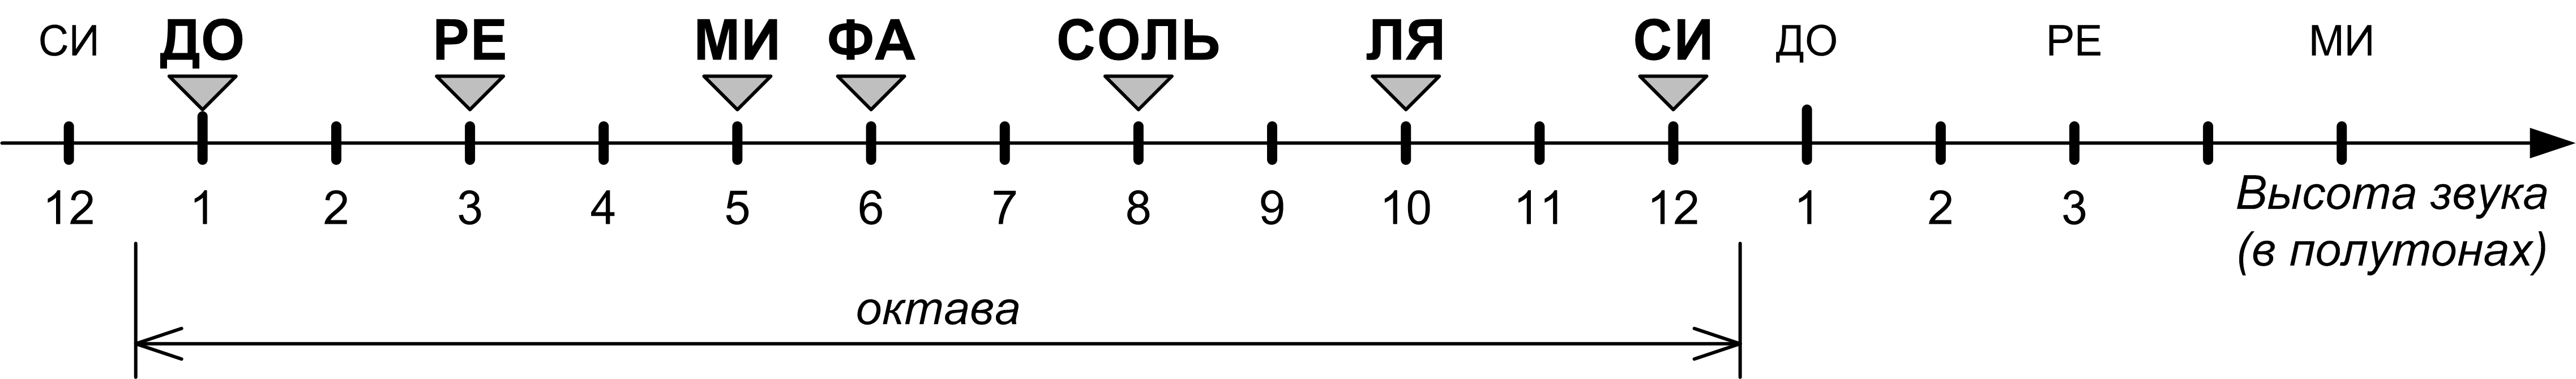
\includegraphics[width=\textwidth]{fig/notes/notes-main-ru} 
    \caption{Названия основных нот октавы RU}\label{fig:notes:names:main:RU}
\end{figure} 

Оставшиеся (12-7)=5 звуков не удостоились отдельных имен. Их имена формируются добавлением суффиксов <<-диез>> или <<-бемоль>> к стоящей по соседству (слева или справа) основной ноте. <<Диез>> повышает звук на полутон, а <<бемоль>> --- понижает. Итак между следующими основными нотами находится <<промежуточный>> звук (см. рисунок \ref{fig:notes:names:all:RU}).
\begin{enumerate}
    \item ДО и РЕ (этот звук может быть назван либо ДО-диез, либо РЕ-бемоль)
    \item РЕ и МИ (РЕ-диез или МИ-бемоль)
    \item ФА и СОЛЬ (ФА-диез или СОЛЬ-бемоль)
    \item СОЛЬ и ЛЯ (СОЛЬ-диез или ЛЯ-бемоль)
    \item ЛЯ и СИ (ЛЯ-диез или СИ-бемоль)
\end{enumerate}

\begin{figure}[!ht]
    \centering
    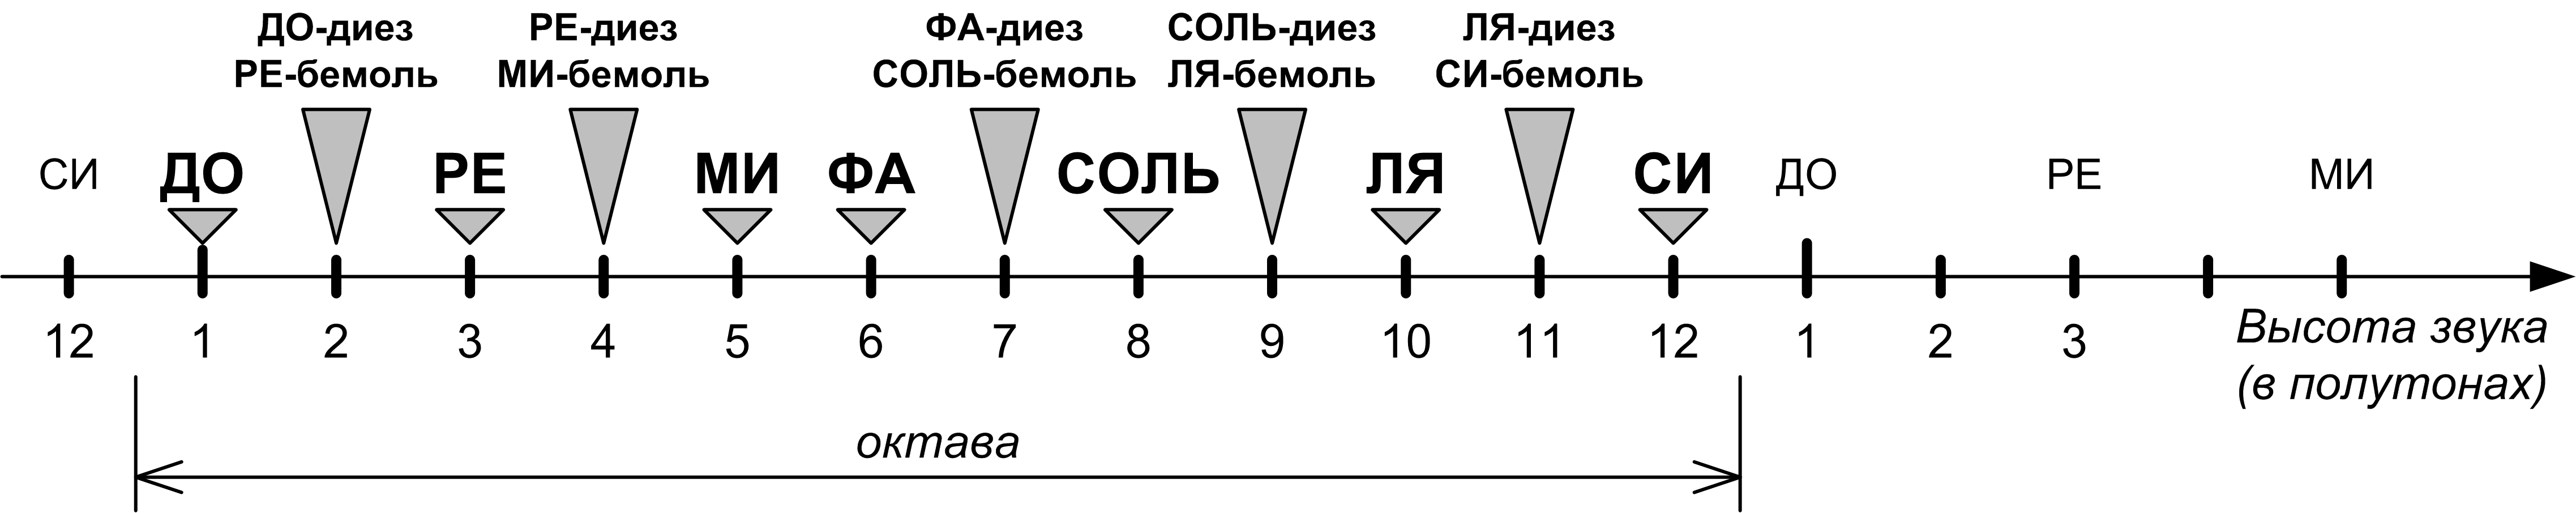
\includegraphics[width=\textwidth]{fig/notes/notes-all-ru} 
    \caption{Названия всех нот октавы RU}\label{fig:notes:names:all:RU}
\end{figure} 

Как видно, <<промежуточные>> ноты могут называться двояко. Какое из имен выбрать? Постараюсь ответить кратко: если вы читаете этот текст и узнаёте для себя что-то новое, то вам позволительно использовать любое\footnote{Это как грамотность в Русском языке: надеть или одеть? Одеть Надежду, надеть одежду! Чужак не осилит. Так что называйте как хотите, знающие друзья поправят, если что. Только помалкивайте на какой-нибудь музыкальной конференции в кругу маститых классических исполнителей}. Все 12 звуков октавы в порядке увеличения высоты:
\begin{center}
    ДО, ДО-диез, РЕ, РЕ-диез, МИ, ФА, ФА-диез, СОЛЬ, СОЛЬ-диез, ЛЯ, ЛЯ-диез, СИ
\end{center}

Когда октаву читают в нисходящем порядке, то грамотно использовать <<-бемоль>>:
\begin{center}
    СИ, СИ-бемоль, ЛЯ, ЛЯ-бемоль, СОЛЬ, СОЛЬ-бемоль, ФА, МИ, МИ-бемоль, РЕ, РЕ-бемоль, ДО
\end{center}

Отметим, что между МИ и ФА, а также между СИ и ДО, промежуточных звуков нет\footnote{Вам уже давно хочется сказать: <<Диез-бемоль! Какого чёрта? Почему? Зачем эти сложности?>> Друзья мои, болею за вас! Творится полный беспредел с точки зрения кодирования! Можно проще, но все привыкли. Знаете, это традиция, в которой есть смысл! Наберитесь терпения}: расстояние между ними --- один полутон. Однако никто не мешает, например, назвать ноту ДО как СИ-диез, или ноту МИ как ФА-бемоль. В устной речи так, конечно, никто не сделает, а вот при записи знаков нот на бумаге такое вполне допустимо, чтобы значки не <<наезжали>> друг на друга.

Американцы и англичане обозначают ноты буквами алфавита (см. также рисунок \ref{fig:notes:names:all:EN}): 
\begin{center}
    A(ля), B(си), C(до), D(ре), E(ми), F(фа), G(соль).
\end{center}

\begin{figure}[!ht]
    \centering
    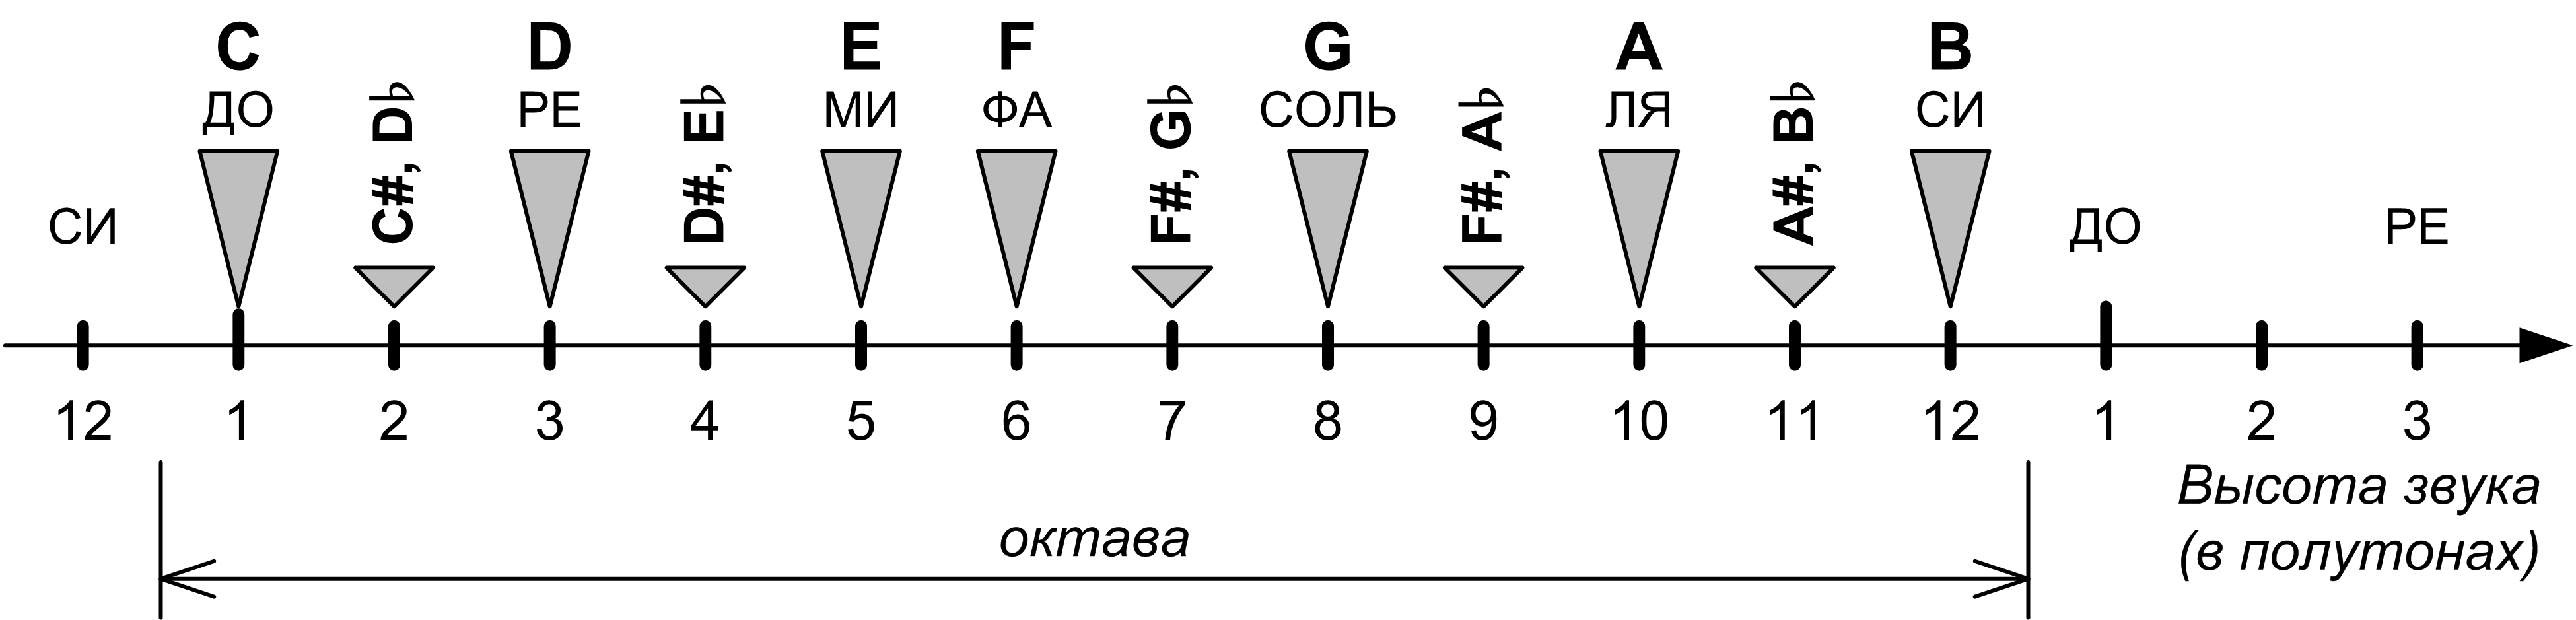
\includegraphics[width=\textwidth]{fig/notes/notes-all-en} 
    \caption{Названия всех нот октавы EN}\label{fig:notes:names:all:EN}
\end{figure} 

Важно запомнить эти обозначения прямо сейчас! Они слишком часто используются в гитарной музыке. Причем вместо суффикса <<-диез>> изпользуется значок $\sharp$, а вместо <<-бемоль>> --- $\flat$. Например, нота ДО-диез может быть обозначена как $C\sharp$ или как $D\flat$.

\begin{Example}[Психоделическая сказочка об английских обозначениях нот]
    И жили они, не тужили с октавой, начинающейся с ЛЯ, то есть, как и положено, c A\ldots Ага, вроде всё логично и просто, как азбука. Английский алфавит читается: A-эй, B-би, C-си, D-ди, E-и, F-эф, G-джи, H-эйч. Как вдруг, в результате спонтанного шизоидного сдвига, всем вдруг стало ясно, что октава должна начинаться с ДО. Причина сего интересна не только психиатрам! Если вы разберетесь с \emph{музыкальным ладом}, то вы сами дадите этому заскоку рациональное объяснение. И порядок немного сломался, ибо стало: CDEFGAB. А потом кому-то показалось, что для ноты СИ буквы не хватило! И назначили для ноты СИ очередную свободную латинскую букву H! Гитаристам с латиницей дело иметь придется часто, поэтому запомните приведенное соответствие и будьте готовы к тому, что для обозначения ноты СИ может быть использована латинская буква H. Все даже чуть сложнее\ldots Если вы увидели книжку, где используется <<H>>, то знайте, что это <<СИ>>. Но не падайте в обморок, если вдруг увидите, что там же используется и латинская <<B>>! В данном клиническом случае <<B>> будет обозначать ноту <<CИ-бемоль>>! Боже упаси!
\end{Example}

Напоследок осталось отметить, что для того, чтобы назвать музыкальный звук, нужно уточнить октаву, к которой он относится. Так как названия нот в пределах октавы повторяются, то октавную систему удобно представлять себе в виде спирали, как на рисунке \ref{fig:notes:names:octave}.

\begin{figure}[!ht]
    \centering
    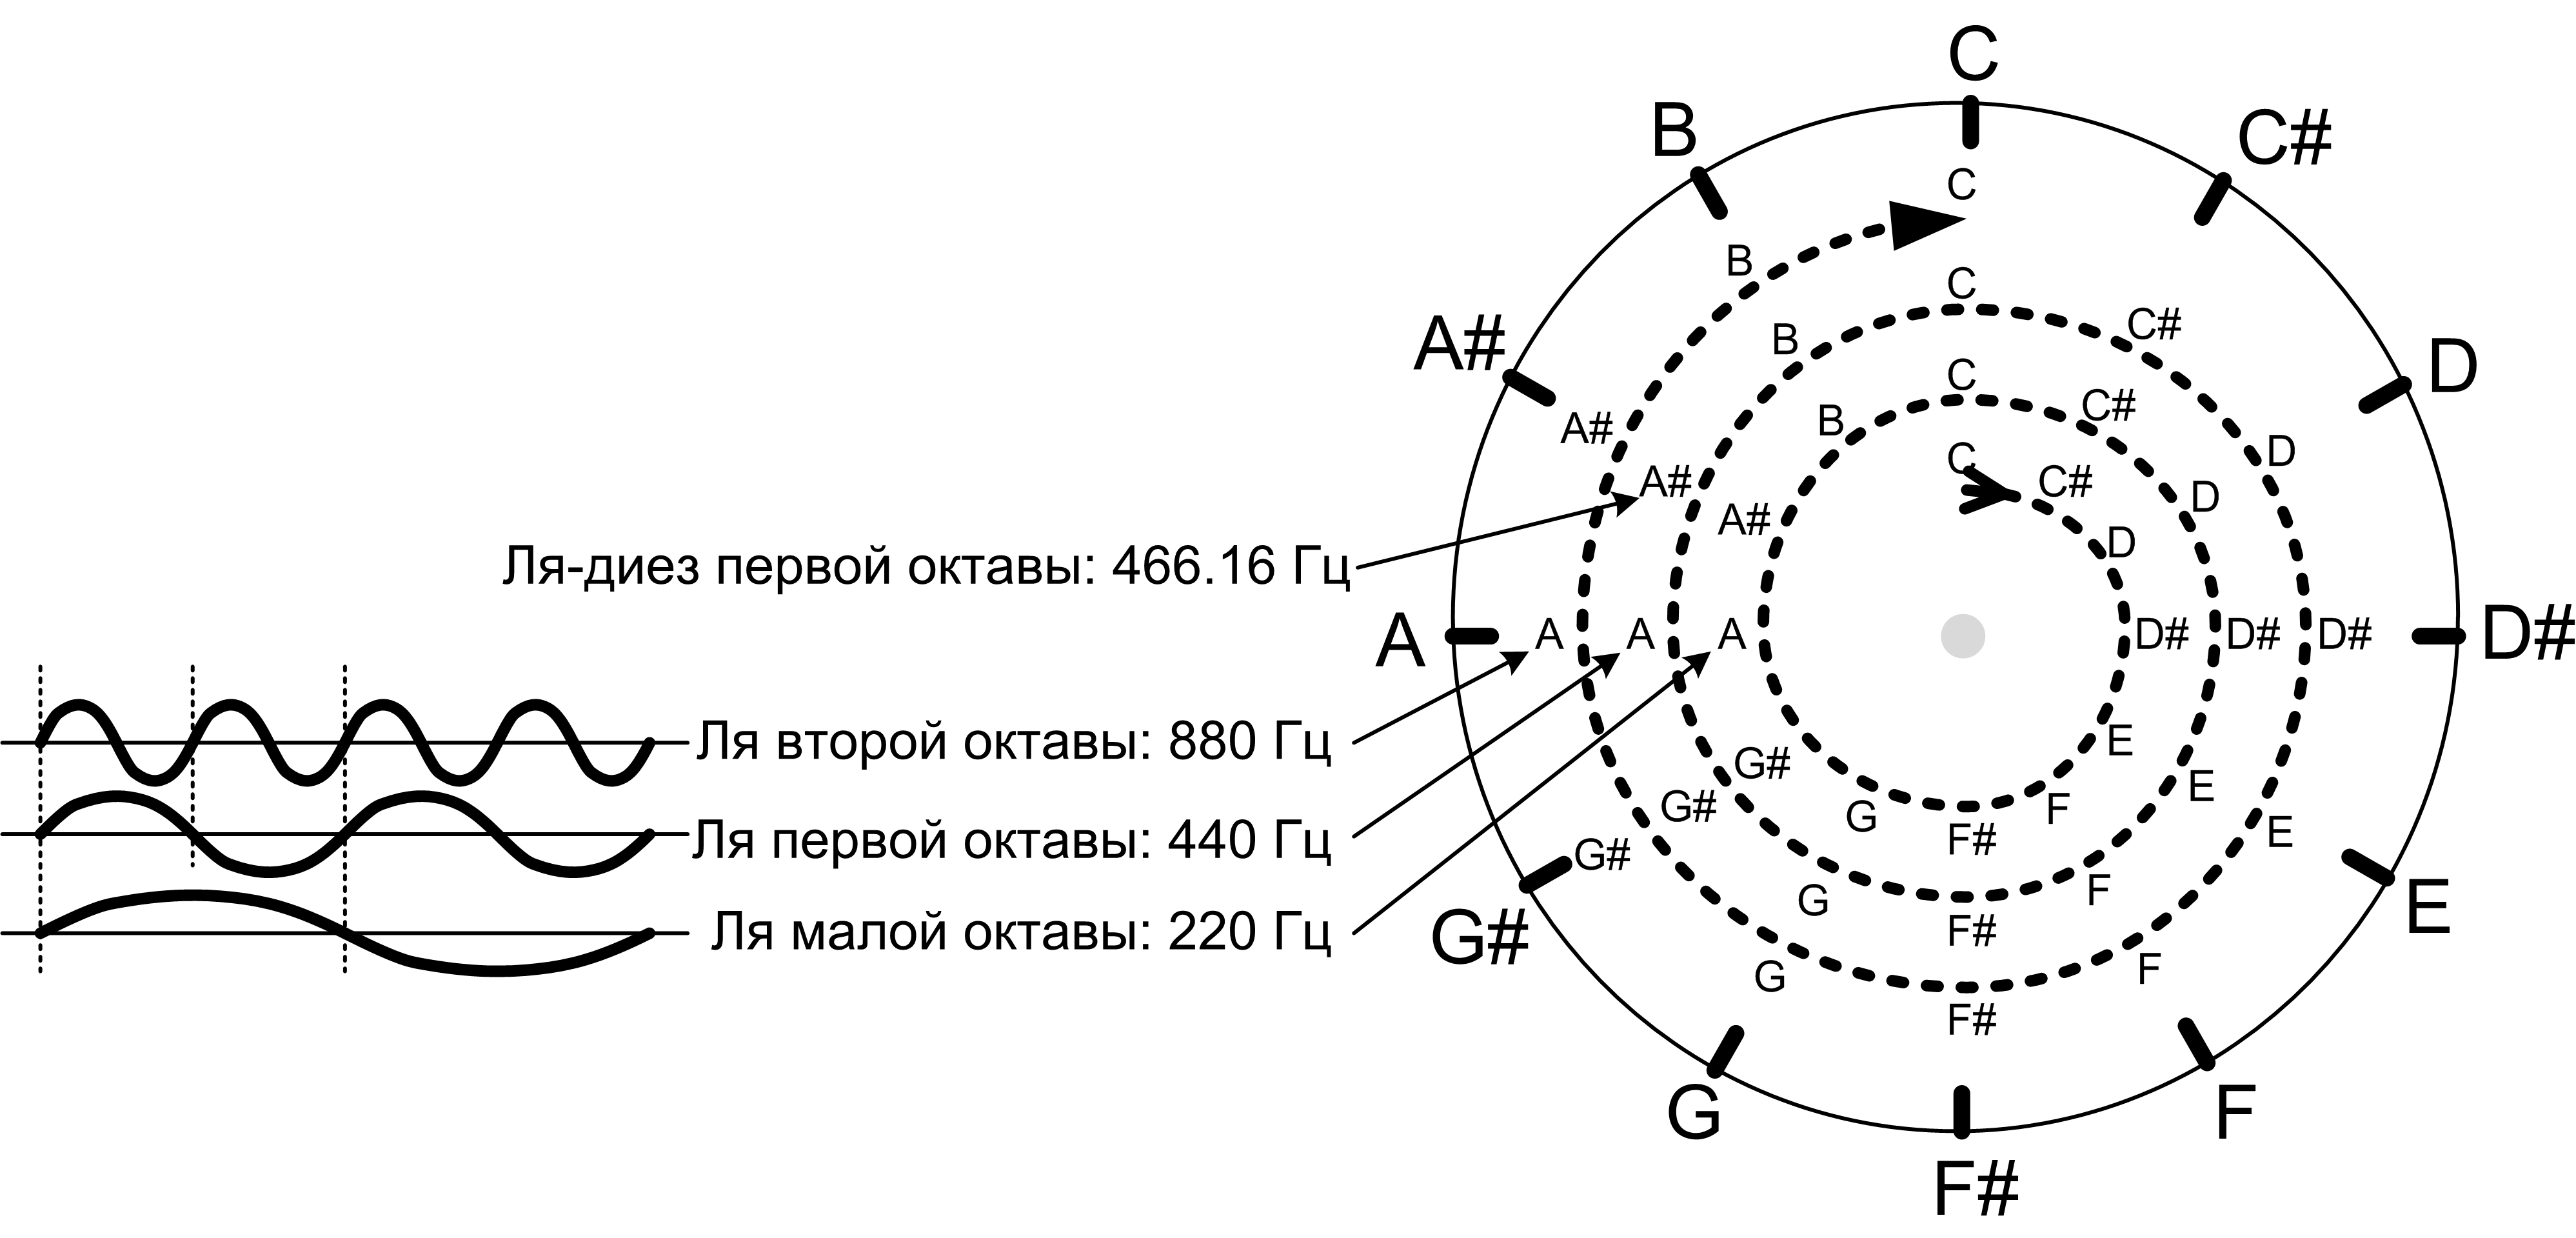
\includegraphics{fig/intervals/octave-spiral} 
    \caption{Пооктавная цикличность музыкальных звуков}\label{fig:notes:names:octave}
\end{figure} 


Названия использующихся в музыке октав приведены в таблице \ref{tab:notes:names:octaves}. Также в таблице приведена частота основного тона входящей в октаву ноты ЛЯ. Частоты остальных нот при желании можно вычислить по формуле \eqref{eq:music:tone:frequency}, надо лишь полутона правильно посчитать. Отдельно \emph{выделены} те октавы, которые входят в диапазон шестиструнной гитары. Справедливости ради следует сказать, что её диапазон звучания полностью включает лишь малую и первую октавы.

\begin{table}[!ht]
    \centering
    \caption{Октавы}
    \label{tab:notes:names:octaves}
    \begin{tabular}{ll}
        \hline\hline
        Название октавы         & Частота ноты Ля, Гц \\
        \hline\hline
        
        Субконтроктава          & 27.5 \\
        Контроктава             & 55   \\
        \emph{Большая октава}   & 110  \\
        \emph{Малая октава}     & 220  \\
        \emph{Первая октава}    & A4=\fbox{440}  \\
        \emph{Вторая октава}    & 880  \\
        Третья октава           & 1760 \\
        Четвертая октава        & 3520 \\
        Пятая октава            & 7040 \\
        \hline
    \end{tabular}
\end{table}

Все же стоит дать краткий ответ на вопрос: <<почему не все 12 нот октавы получили индивидуальные имена?>>. Дело в том, что из <<основных>> нот можно составить гармоничную мелодию, а <<промежуточные>> ноты при этом будут использоваться крайне редко. За подробным ответом пожалуйте в царство гармонии, в раздел \ref{ch:harmony}.


\section{Что тут зашифровано? Запись нот}

Чтобы записать ноты, купите нотную тетрадь или на обычном листе начертите нотоносец --- пять параллельных, расположенных друг под другом через равные интервалы (около двух миллиметров) линий:
 

Традиционно ноты для шестиструнной гитаре записываются в скрипичном ключе, который своим хвостиком огибает вторую снизу линию нотоносца, на которой располагется СОЛЬ \emph{малой} октавы\footnote{Для других музыкальных инструментов, в первую очередь, для фортепиано, скрипичный ключ показывает положение СОЛЬ \emph{первой} октавы, но для гитары, чтобы использовать один нотоносец, ноты пишут на <<фортепианный>> скрипичный нотоносец на октаву выше.}.

\section{Как это сыграть на гитаре? Гитарная табулатура}



%TODO ритм и переборы